%%%%%%%%%%%%%%%%%%%%%%%%%%%%%%%%%%%%%%%%%%%%%%%%%%%%%%%%%%%%%%%%%%%%%%%%%%%%%%
%%%%%%%%%%%%%%%%%%%%%%%%%%%%%%%%%%%%%%%%%%%%%%%%%%%%%%%%%%%%%%%%%%%%%%%%%%%%%%
%%
%% Dokumentace k interpretu jazyka IFJ14, 2014
%%
%% Upravená původní dokumentace od Davida Martinka.
%%%%%%%%%%%%%%%%%%%%%%%%%%%%%%%%%%%%%%%%%%%%%%%%%%%%%%%%%%%%%%%%%%%%%%%%%%%%%%
%%%%%%%%%%%%%%%%%%%%%%%%%%%%%%%%%%%%%%%%%%%%%%%%%%%%%%%%%%%%%%%%%%%%%%%%%%%%%%
\documentclass[12pt,a4paper,titlepage,final]{article}

% cestina a fonty
\usepackage[slovak]{babel}
\usepackage[utf8]{inputenc}
% balicky pro odkazy
\usepackage[bookmarksopen,colorlinks,plainpages=false,urlcolor=blue,unicode]{hyperref}
\usepackage{url}
\usepackage{amsmath}
\usepackage{capt-of}
\usepackage[Q=yes]{examplep}
\usepackage{enumitem}

% obrazky
\usepackage{graphicx}
% velikost stranky
\usepackage[text={15.2cm, 25cm}, ignorefoot]{geometry}



\begin{document}

%%%%%%%%%%%%%%%%%%%%%%%%%%%%%%%%%%%%%%%%%%%%%%%%%%%%%%%%%%%%%%%%%%%%%%%%%%%%%%
% titulní strana
\begin{titlepage}

\vspace*{2cm}
\begin{figure}[!h]
  \centering
  \includegraphics[width=10cm]{img/logo.eps}
\end{figure}

\vfill

\begin{center}

\begin{Huge}
  Model dopravního uzlu
\end{Huge}

\bigskip

\begin{Large}
  Modelování a simulace
\end{Large}

\bigskip

\begin{Large}
	2015/2016
\end{Large}

\end{center}

\vfill

\begin{center}
\begin{Large}
\today
\end{Large}
\end{center}

\vfill

\begin{flushleft}
\begin{normalsize}
\begin{tabular}{ll}
\bf Riešitelia:\hspace{3mm} & Peter Gazdík (\url{xgazdi03@stud.fit.vutbr.cz}) \\
& Andrej Baáš (\url{xbaasa00@stud.fit.vutbr.cz}) \\[3mm]

& Fakulta Informačních Technologií \\
& Vysoké Učení Technické v~Brně
\end{tabular}
\end{normalsize}
\end{flushleft}
\end{titlepage}


%%%%%%%%%%%%%%%%%%%%%%%%%%%%%%%%%%%%%%%%%%%%%%%%%%%%%%%%%%%%%%%%%%%%%%%%%%%%%%
% obsah
\pagestyle{plain}
\pagenumbering{roman}
\setcounter{page}{1}
\tableofcontents

%%%%%%%%%%%%%%%%%%%%%%%%%%%%%%%%%%%%%%%%%%%%%%%%%%%%%%%%%%%%%%%%%%%%%%%%%%%%%%
% textova zprava
\newpage
\pagestyle{plain}
\pagenumbering{arabic}
\setcounter{page}{1}

%%%%%%%%%%%%%%%%%%%%%%%%%%%%%%%%%%%%%%%%%%%%%%%%%%%%%%%%%%%%%%%%%%%%%%%%%%%%%%%%
\section{Úvod}
%%%%%%%%%%%%%%%%%%%%%%%%%%%%%%%%%%%%%%%%%%%%%%%%%%%%%%%%%%%%%%%%%%%%%%%%%%%%%%%%

Tento dokument popisuje vytváranie modelu~\cite[str.\,6]{opora} a následnú simuláciu~\cite[str.\,7]{opora} dopravného uzla,
konktrétne železničnej stanice Púchov na Slovensku. Cieľom práce je simuláciou
overiť správnosť návrhu grafikonu vlakovej dopravy~\cite{wiki:gvd} (GVD) pre rok
2015/2016, ktorý vstupuje do platnosti 13.\,12.\,2015. Platnosť budeme overovať na základe skúmania, ako často dochádza k zmene pridelenia koľají dispečerom oproti pomôcke \uv{Plán obsadenia dopravných koľají}~\cite[str.\,9]{szdc_d6}, ktorá stanovuje pre každý vlak koľaj, na ktorú by mal za ideálnych podmienok prísť.
%-------------------------------------------------------------------------------
\subsection{Autori a zdroje}
%-------------------------------------------------------------------------------

Na vypracovaní projektu sa podielali študenti FIT VUT Andrej Baáš a Peter Gazdík.
Autori využívali konzultácie so zamestnancom Železníc Slovenskej republiky (ŽSR)
Ing.~Jozefom Baášom, ktorý pracuje ako vedúci technického oddelenia a autorom taktiež
poskytol niektoré odborné fakty, ktoré boli k vypracovaniu projektu nevyhnutné.

Medzi hlavné zdroje informácii patrila študijná opora~\cite{opora} k predmetu
Modelovanie a simulácie, schéma koľajiska na žel. stanici Púchov~\cite{kolaje},
Plán obsadenia koľají na žel. stanici Púchov~\cite{pok}, Grafikony vľakovej
dopravy~\cite{gvd106}\cite{gvd125} zachycujúce pohyb vlakov v stanici Púchov a
množstvo ďalšej literatúry zaoberajúcej sa riadením a simuláciou dopravy na železnici,
ktorá bude priebežne spomínaná v texte.

\begin{figure}[h]
	\centering
	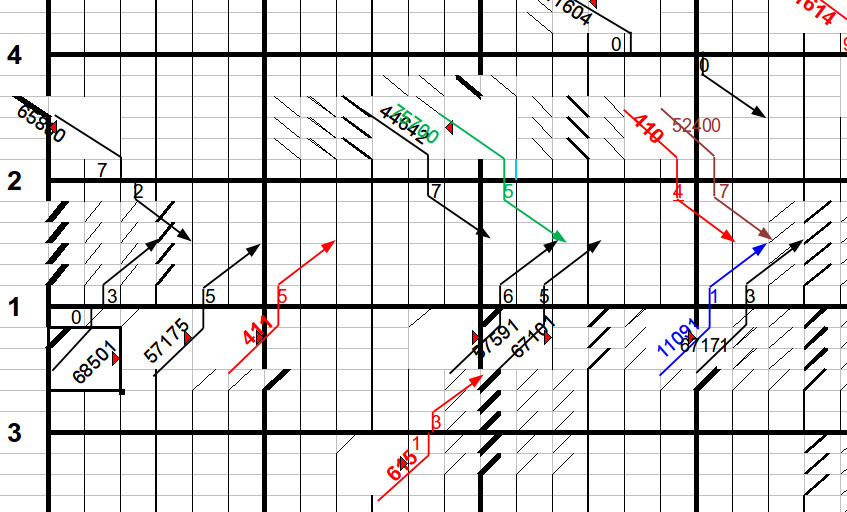
\includegraphics[width=0.8\textwidth]{img/pok}
	\caption{Ukážka plánu obsadenia dopravných koľají} \label{fig:pok_example}
\end{figure}

\begin{figure}
	\centering
	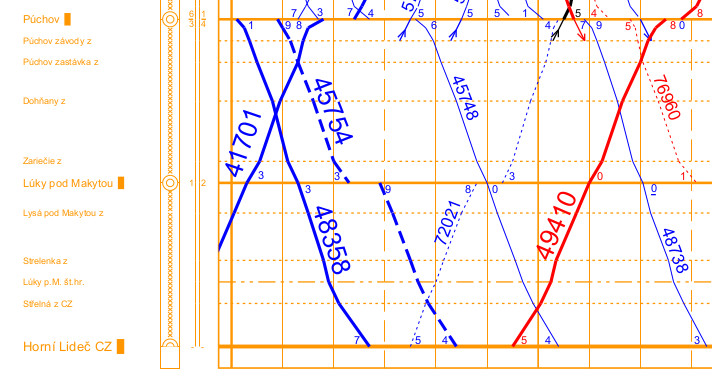
\includegraphics[width=0.8\textwidth]{img/gvd}
	\caption{Ukážka grafickej podoby GVD} \label{fig:gvd_example}
\end{figure}


%-------------------------------------------------------------------------------
\subsection{Prostredie pre overovanie validity modelu}
%-------------------------------------------------------------------------------

Nakoľko modelovaný systém ešte v súčasnej podobe nie je možné sledovať (v čase modelovania~\cite[str.\,6]{opora} ešte neprišiel do platnosti nový grafikon vlakovej dopravy), bolo overovanie validity~\cite[str.\,15]{opora} vykonávané len porovnávaním výstupu modelu s očakávaným správaním reálneho systému~\cite[str.\,6]{opora}.
Očakávané správanie reálneho systému bolo pre nás dané práve pomocou GVD.
Na základe toho, že výstup modelu pri behu bez zavedených meškaní verne kopíroval návrh GVD
usudzujeme, že model bez zavedených meškaní je validný.

Posúdiť validitu modelu so zavedenými meškaniami nebolo možné jednoznačne. Vychádzame
len z predpokladu, že nakoľko nedošlo oproti súčasnému GVD k výrazným zmenám v pohybe
vlakov, tak výstup z našeho modelu pri meškaní zodpovedajúcom prevádzke podľa súčasného GVD bude vykazovať podobné chovanie ako súčasný reálny systém. Výsledok
tohto experimentu zodpovedal osobným skúsenostiam dispečerov riadiacich dopravu v stanici Púchov (nevedú sa totiž štatistiky o zmene priradenia koľají) a teda taktiež považujeme náš model aj v tomto ohľade za validný.

%%%%%%%%%%%%%%%%%%%%%%%%%%%%%%%%%%%%%%%%%%%%%%%%%%%%%%%%%%%%%%%%%%%%%%%%%%%%%%%%
\section{Rozbor témy a použitých metód/technológií} \label{sec:rozbor}
%%%%%%%%%%%%%%%%%%%%%%%%%%%%%%%%%%%%%%%%%%%%%%%%%%%%%%%%%%%%%%%%%%%%%%%%%%%%%%%%

Železničná stanica Púchov je tvorená celkovo 15 koľajami~\cite{kolaje},
pričom len 4 z nich sa nachádzajú pri nástupištiach a je ich teda možné využiť
pre nástup a výstup pasažierov (koľaje č. 3,4,7,8). Dĺžka nástupišť je vo všetkých prípadoch rovnaká~\cite{kolaje}, a to 400m, takže je na nich možné obslúžiť všetky vlaky, ktoré v tejto stanici zastavujú. Koľaje č. 1 a 2 slúžia len na prejazd vlakov cez stanicu a zvyšné koľaje
slúžia na odstavenie vlakov stojacich v stanici dlhšiu dobu (nákladné vlaky a vlaky,
ktoré v stanici zostávajú cez noc). Spomínané koľaje je možné vidieť aj na obrázku č.~\ref{fig:kolaje}.

\begin{figure}[h]
	\centering
	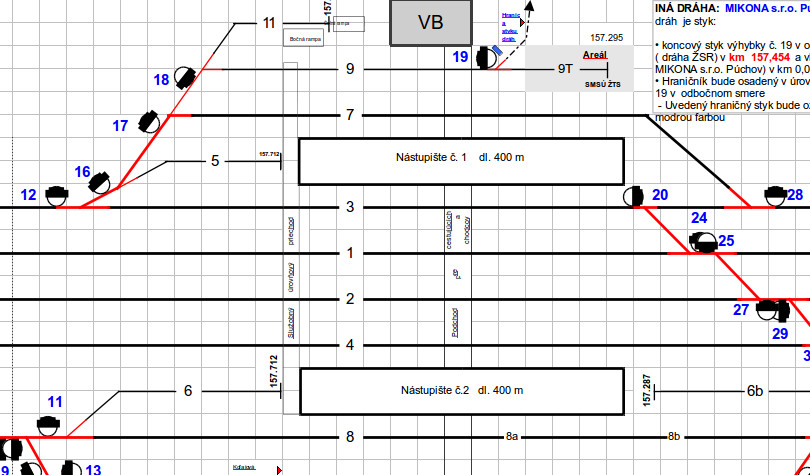
\includegraphics[width=0.9\textwidth]{img/kolaje}
	\caption{Výrez zo schémy koľají ŽST Púchov} \label{fig:kolaje}
\end{figure}

Vlaky prichádzajú do stanice v ideálnom prípade v časoch daných cestovným poriadkom alebo s určitým meškaním oproti cestovnému poriadku. Vychádzajúc zo štatistiky ŽSR~\cite{meskanie} v odbobí od 11.\,2.\,2015 do 12.\,2.\,2015 bolo zmeškaných 20.23\,\% vlakov s priemerným meškaním 11.96~min.

Vlaku prichádzajúcemu na nástupište je dispečerom riadiacim dopravu v danej stanici
určená koľaj na základe Plánu obsadenia dopravných koľají~\cite{pok} a umožnený
príjazd vlaku na túto koľaj nastavením výhybiek do príslušnej polohy a nastavením
príslušných návestidiel~\cite{riadenie}. V prípade mimoriadnosti (meškanie vlaku, výluka koľaje),
kedy je koľaj daná Plánom obsadenia koľají nedostupná, dochádza k prideľeniu náhradnej
koľaje~\cite{dispecer}.

Nakoľko však takéto zmeny vyžadujú množstvo úkonov, ktoré musí dispečer vykonať,
je žiaduce, aby bol plán obsadenia koľají navrhnutý s ohľadom na možné mimoriadnosti (najmä meškania). Z tohoto dôvodu sa bude táto práca
zaoberať simuláciou~\cite[str.\,7]{opora} Plánu obsadenia koľají pre rok 2015/2016, ktorý od 13.\,12.\,2015 prichádza
do platnosti, na odolnosť voči meškaniam.

Po pridelení koľaje následne vlak zastaví v stanici do doby pravidelného odjazdu, alebo
v prípade, že sa jedná o zmeškaný vlak a doba státia v stanici by mala byť kratšia ako minimálny čas potrebný na odbavenie vlaku, tak vlak stojí v stanici tento minimálny čas. Minimálny čas bol určovaný na základe
plánu obsadenia koľají a pre jednotlivé vlaky sa líši v závislosti na tom, či vlak v stanici
zastavuje len na čas potrebný pre výstup a nástup pasažierov alebo tento vlak v stanici končí a
dochádza pri ňom k úkonom potrebným na zaistenie jeho opätovného vypravenia na iný spoj (upratovanie, prestavenie rušňa na druhý koniec vlaku atď.).

Výnimkou sú vlaky kategórie IC, ktoré v stanici nezastavujú a len ňou prechádzajú konštantnou rýchlosťou.
Pozorovaním v stanici sme zmerali, že tieto vlaky prejdú cez stanicu za 15~sekúnd.

Vlaky, ktoré v stanici jazdu končia a odchádzajú až o niekoľko hodín sú prestavené na koľaj,
kde neobmedzujú pohyb ďalších vlakov v stanici. Spravidla sú teda odstavené na
niektorú odstavnú koľaj.

Vlak môže zo stanice odísť neskôr ako je jeho plánovaný čas odjazdu aj v prípade,
že tento vlak je plánovaný ako prípojný a čaká v stanici na prípoj maximálne po
dobu danú čakacím časom~\cite[str.\,3]{pripoje}, ktorá začne plynúť od času jeho pravidelného odjazdu.
Po príchode prípoja je taktiež potrebné zohľadniť dobu potrebnú na prestup
cestujúcich. Prípojné vlaky v stanici Púchov majú štandardné čakacie doby stanovené
všeobecnými predpismi~\cite{pripoje}, ktoré udávajú pre prípojné vlaky kategórie Ex, R čakacie
časy 5\,minút a pre vlaky kategórie Os 10~minút.

Vlak môže byť zo stanice vypravený na odjazdovú koľaj až v okamžiku, kedy pred ním vypravený vlak
na túto koľaj urazil bezpečnú vzdialenosť od prvého návestidla~\cite{riadenie}
(daná zábrzdnou vzdiaľenosťou vychádzajúcej z maximálnej traťovej rýchlosti). Z tejto
vzdialenosti je potom možné určiť dobu, počas ktorej sú odjazdové koľaje zo stanice
obsadené. Tieto časy sú potom nasledovné (výpočet vykonával zamestnanec ŽSR a nemáme ich k dispozícii): pre smer Praha 2~min.~23~sekúnd, smer Bratislava 2~min.~32~sekúnd a smer Košice 1~minúta.

%-------------------------------------------------------------------------------
\subsection{Popis použitých postupov}
%-------------------------------------------------------------------------------

Model bol implementovaný v jazyku C++ využítím knižnice SIMLIB~\cite{simlib}, ktorá
poskytuje základné prostriedky pre popis diskrétnych modelov~\cite[str.\,12]{opora}. Zároveň je však možné používanie všetkých ostatných prostriedkov jazyka C++ a je tak možné rozšíriť knižnicu o ďalšie prostriedky potrebné pre modelovanie.

Preklad a testovanie programu prebiehalo na školskom serveri \url{merlin.fit.vutbr.cz} pod
operačným systémom CentOS 6.7 s prekladačom GCC vo verzii 4.9.3.

%-------------------------------------------------------------------------------
\subsection{Popis pôvodu použitých metód}
%-------------------------------------------------------------------------------

Použitá simulačná knižnica SIMLIB bola získaná z oficiálnych stránok a jej používanie
je možné podľa podmienok licencie GNU LGPL.

%%%%%%%%%%%%%%%%%%%%%%%%%%%%%%%%%%%%%%%%%%%%%%%%%%%%%%%%%%%%%%%%%%%%%%%%%%%%%%%%
\section{Koncepcia}
%%%%%%%%%%%%%%%%%%%%%%%%%%%%%%%%%%%%%%%%%%%%%%%%%%%%%%%%%%%%%%%%%%%%%%%%%%%%%%%%

Pri modelovaní koľajiska v stanici uvažujeme len koľaje č. 1,2,3,4,7,8, pretože
zvyšné koľaje sú využívané primárne na odstavenie vlakov a nie sú
zahrnuté v pláne obsadenia dopravných koľají.

Taktiež v nami vytvorenom modeli neuvažujeme pohyb nákladných vlakov cez stanicu,
nakoľko tieto vlaky majú pri riadení dopravy najnižšiu prioritu~\cite[str.\,342]{riadenie}
a pri meškaní vlakov prechádzajú stanicou tak, aby neobmedzili pohyb osobných vlakov s vyššou mierou priority.

Zanedbávané sú aj výhybky v stanici, ktorých úlohou je zabezpečiť príjazd vlakov
na pridelenú koľaj. Model toto zabezpečuje na abstraktnejšej úrovni. Čas prechodu výhybkami
je zahrnutý do doby, po ktorú vlak obsadzuje odjazdovú a príjazdovú koľaj.

%-------------------------------------------------------------------------------
\subsection{Spôsob vyjadrenia konceptuálneho modelu}
%-------------------------------------------------------------------------------

% V skratke zhrnúť nami vytvorené petriho siete a čo znázorňujú,
% ich detailnejší popis až ďalšej kapitole

Všetky navrhnuté petriho siete~\cite[str.\,31]{opora} zobrazujú model s veľkou mierou abstrakcie, nakoľko
správanie systému je podmienené množstvom rozhodovacích algoritmov, ktoré by bolo
petriho sieťou obtiažne modelovať.

Príjazdové a odjazdové koľaje sú znázornené petriho sieťou na obrázku \ref{fig:inouttrack}. Generovanie vlakov, ktoré petriho sieť zobrazuje, je zjednodušené a bližšie je popísané v kapitole \ref{sec:generovanie}.

Príjazd, zabratie a odjazd vlaku z koľaje v stanici vyobrazuje petriho sieť na obrázku \ref{fig:track}. Je na nej možné vidieť dve obslužné linky s výlučným prístupom~\cite[str.\,36]{opora}, pričom jedna reprezentuje dispečera v stanici a druhá koľaj v stanici.

Pri modelovaní celej stanice Púchov je potrebné využiť celkovo 3 príjazdové a 3 odjazdové koľaje pre smer Bratislava, Košice, Praha a 6 koľají v stanici, pričom pre všetky tieto koľaje bude slúžiť len jedna obslužná linka dispečera.

%-------------------------------------------------------------------------------
\subsection{Popis konceptuálneho modelu}
%-------------------------------------------------------------------------------

% detailne popísať jednotlivé časti petriho siete a na koniec do detailu slovne
% popísať činnosť dispečera pri prideľovaní koľaje a stanovení meškania vlaku

\subsubsection*{Príjazdové a odjazdové koľaje a generovanie vlakov} \label{sec:generovanie}

Príjazdová a odjazdová koľaj vyobrazená na obrázku \ref{fig:inouttrack} predstavuje obslužnú
linku s výlučným prístupom~\cite[str.\,36]{opora}. Po zabraní linky prichádzajúcim, resp. odchádzajúcim vlakom vlak obsadí túto linku na dobu závislú na parametroch kontrétnej koľaje (dĺžka, traťová rýchlosť), viď kapitola \ref{sec:rozbor}.

\begin{figure}[!h]
	\centering
	\includegraphics[width=0.5\textwidth]{img/inouttrack}
	\caption{Petriho sieť: Príjazdová a odjazdová koľaj} \label{fig:inouttrack}
\end{figure}

Vlaky sú na príjazdovú koľaj generované v časoch daných cestovným poriadkom, pričom ale tieto vlaky môžu nadobúdať meškanie stanovené na základe metodiky DB~Richtlinie 405.0204A03~\cite[str.\,11]{studie_mas}.

\vspace{1em}
{\setlength{\parindent}{0cm}
Algoritmus generovania meškania podľa tejto metodiky je následovný:
\begin{itemize}
	\item vzhľadom ku pravdepodobnosti sa zistí, či vlak bude zmeškaný alebo nie,
	\item ak nie, vlak nebude omeškaný,
	\item ak áno, vygeneruje sa meškanie dané exponenciálnym rozdelením so stanovenou
	strednou hodnotou.
\end{itemize}
}

\subsubsection*{Koľaje v stanici}

Každá koľaj v stanici je reprezentovaná obslužnou linkou s výlučným prístupom, viď obrázok \ref{fig:track}.
Koľaj umožňuje príjazd vlaku v obidvoch smeroch. Pred obsadením koľaje vlakom najskôr dôjde k zabratiu linky \textit{Dispečer}, ktorý prichádzajúcemu vlaku pridelí koľaj a následne sa tento vlak pokúsi túto koľaj obsadiť. Situácia, že by bola koľaj aj napriek prideleniu dispečerom obsadená a vlak by na ňu musel čakať pred stanicou by znamenala, že všetky koľaje vhodné pre daný vlak sú už obsadené inými vlakmi.

\begin{figure}[!h]
	\centering
	\includegraphics[width=0.8\textwidth]{img/track}
	\caption{Petriho sieť: Koľaj v stanici spolu s dispečerom} \label{fig:track}
\end{figure}

Vlak následne obsadí koľaj do doby pravidelného odjazdu alebo na minimálnu dobu potrebnú pre odbavanie vlaku, ktorá je určená pre konkrétny vlak.

Po tejto dobe môže vlak opustiť koľaj, ale len v prípade, že je voľná odjazdová koľaj v smere odjazdu vlaku.
Ak tomu tak nie je, vlak obsadzuje koľaj v stanici až do doby uvoľnenia odjazdovej koľaje.

\subsubsection*{Stanovenie doby státia vlaku v stanici} \label{sec:statie}

Pri príjazde vlaku do stanice je potrebné určiť dobu čakania, po ktorú má vlak v stanici stáť. Túto činnosť zabezpečuje v reálnom systéme dispečer riadenia dopravy. V modelovanom systéme však táto činnosť musí byť zabezpečená vhodne navrhnutým algoritmom.

Pri určovaní doby, ktorú má vlak stáť v stanici rozlišujeme následovné situácie:
\begin{enumerate}
	\item vlak prichádza včas, prípadne s takým malým meškaním, že je možné jeho vypravenie v čase pravidelného odjazdu,
	\item vlak prichádza zmeškaný a nie je ho možné stihnúť vypraviť v čase pravidelného odjazdu,
	\item vlak je plánovaný ako prípojný a musí čakať na zmeškaný prípoj podobu čakacieho času.
\end{enumerate}

V prípade bodu 1 a 2 stačí určiť dobu, ktorá je daná rozdielom
času pravidelného odjazdu a skutočného príjazdu a v prípade, že je táto doba kratšia
ako minimálna doba potrebná na odbavenie vlaku v stanici, tak tento vlak čaká minimálne po túto dobu, inak do času odjazdu.

V 3. bode je potrebné pri rozhodovaní uvažovať aj tzv. čakací čas, viď. kapitola \ref{sec:rozbor},
po ktorý vlak čaká v stanici na prípoj, ktorý je dôsledkom meškania oneskorený a tatiež čas potrebný na prestup cestujúcich. Situáciu bližšie popisujú obrázky \ref{fig:prip_bez} a \ref{fig:prip_s}.

Obrázok \ref{fig:prip_bez} znázorňuje prípad, kedy vlak $r_i$ prichádza do stanice v čase plánoveného príjazdu $t_{Pa}$ a prípojný vlak $r_j$ odchádza v čase plánovaného odjazdu $t_{Pd}$. Čas $T_c$ reprezentuje čas potrebný na prestup cestujúcich z vlaku $r_i$ na vlak $r_j$ a čas $T_w$ je čakací čas.

\begin{figure}[!h]
	\vspace{2em}
	\centering
	\includegraphics[width=0.6\textwidth]{img/pripoj_bezmeskania}
	\caption{Vzťah medzi prichádzajúcim a prípojným vlakom bez meškania} \label{fig:prip_bez}
\end{figure}

Na obrázku \ref{fig:prip_s} je potom vyobrazený prípad, kedy je vlak $r_i$ zmeškaný a prichádza do stanice
v čase $t_{Ra}$, následne dochádza k prestupu cestujúcich po dobu $T_c$ a odjazdu prípojného vlaku
v čase $t_{Rd}$. Ak by čas príchodu $t_{Ra}$ vlaku $r_i$ bol v takom okamžiku, že doba $T_c$ zasahuje až za koniec čakacej doby $T_w$, prípojný vlak $r_j$ čaká aj v takomto prípade.

\begin{figure}[!h]
	\vspace{2em}
	\centering
	\includegraphics[width=0.6\textwidth]{img/pripoj_smeskanim}
	\caption{Vzťah medzi zmeškaným prichádzajúcim vlakom a prípojným vlakom} \label{fig:prip_s}
\end{figure}

\vspace{1em}
{\setlength{\parindent}{0cm}
Činnosť algoritmu pre stanovenie čakacieho času je teda nasledovná:
\begin{itemize}
	\item ak vlak nie je prípojný, stanov dobu čakania na základe doby odjazdu, ale minimálne na dobu
	danú minimálnym časom potrebným pre odbavenie, inak pokračuj,
	\item ak vlak je prípojný a vlak, na ktorý čaká už prišiel do stanice, stanov dobu čakania rovnako ako v prechádzajúcom bode, inak pokračuj,
	\item zisti, či vlak, na ktorý vlak čaká príde ešte pred uplynutím čakacej doby, ak áno, stanov dobu čakania vlaku v stanici s ohľadom na príchod tohoto vlaku a času potrebného na prestup cestujúcich.
\end{itemize}
}

\subsubsection*{Prideľovenie koľaje} \label{sec:pridelovanie}

Algoritmus nahradzujúci činnosť dispečera zároveň stanovuje koľaj, ktorú má vlak pri príjazde obsadiť.

Najjednoduchšia situácia nastáva v prípade, kedy je koľaj, ktorú má prichádzajúci vlak pridelenú
podľa plánu obsadenia koľají, voľná a dôjde k prideleniu práve tejto koľaje.

V prípade, že je táto koľaj obsadená, snaží sa algoritmus o pridelenie inej koľaje na základe výpočtu hodnotiacej funkcie pre každú koľaj. Hodnotiaca funkcia zohľadňuje aktuálne obsadenie koľají,
plánované obsadenie koľají v ďalšiom časovom období a taktiež smer jazdy, pre ktorý je koľaj primárne určená (nie je príliš dôležité) a v neposlednom rade, či je koľaj pri nástupišti, ak vlak zastavuje v stanici.

\vspace{1em}
{\setlength{\parindent}{0cm}
Pri prideľovaní koľaje teda algoritmus postupuje nasledujúcim postupom:
\begin{itemize}
	\item ak je koľaj daná Plánom pridelenia koľají voľná, prideľ prichádzajúcemu vlaku
	túto koľaj a skonči,
	\item ak takto určená koľaj nie je voľná, vypočítaj hodnotiacu funkciu podľa kritérii vyššie pre všetky koľaje a prideľ koľaj s najlepším výsledkom.
\end{itemize}
}

%%%%%%%%%%%%%%%%%%%%%%%%%%%%%%%%%%%%%%%%%%%%%%%%%%%%%%%%%%%%%%%%%%%%%%%%%%%%%%%%
\section{Architektúra simulačného modelu/simulátoru}
%%%%%%%%%%%%%%%%%%%%%%%%%%%%%%%%%%%%%%%%%%%%%%%%%%%%%%%%%%%%%%%%%%%%%%%%%%%%%%%%

Kapitola popisuje implementáciu konceptuálneho modelu v jazyku C++ s využitím knižnice
SIMLIB.

%-------------------------------------------------------------------------------
\subsection{Mapovanie abstraktného modelu do simulačného modelu}
%-------------------------------------------------------------------------------

Koľaje v stanici sú reprezentované triedou \texttt{Track}, odjazdové a príjazdové koľaje triedou \texttt{InOutTrack}, dispečer v stanici triedou \texttt{Dispetcher}. Všetky tieto triedy dedia od triedy \texttt{Facility}, ktorá definuje obslužnú linku s výlučným prístupom.

Vlaky reprezentuje trieda \texttt{Train}. Generovanie vlakov zabezpečuje trieda
\texttt{Generator} a nastavuje im rôzne parametre, ktoré sú načítavané zo súboru vo formáte CSV.
Popis týchto parametrov sa nachádza v ďalšej kapitole. \texttt{Generator} vygeneruje
vlaky zodpovedajúce jednomu dňu (resp. časti dňa, ak simulujeme kratší časový úsek) a následne
sa aktivuje až o čas, ktorý reprezentuje tento úsek. Pri generovaní zároveň ukladá
informácie o vygenerovaných vlakoch a ich časoch do objektu triedy \texttt{MyCalendar}, ktorý
v zjednodušenej podobe slúži ako kalendár udalostí, ako ho poznáme z knižnice SIMLIB.

\texttt{Dispetcher}, ktorý zabezpečuje prideľovanie koľají a nastavovanie časov čakania procesom \texttt{Train} využíva práve spomínaný kalendár na získanie skutočných príjazdov vlakov v budúcnosti, ktoré potrebuje pre jeho činnosť.

\subsubsection{Formát vstupného súboru}

Väčšina údajov, ktoré sú potrebné pri behu simulácie je načítavaných zo súboru vo formáte CSV.
Sú v ňom obsiahnuté údaje získané z GVD a plánu obsadenia koľají. Konkrétne následovné:

\begin{itemize}
	\item kategória vlaku - Os, R, Ex, IC,
	\item číslo vlaku,
	\item plánovaný príchod zadaný v minútach od začiatku dňa (00:00 = 0, 01:00 - 60 atď.),
	\item plánovaný odchod,
	\item minimálna doba potrebná na zaistenie odbavenia vlaku v stanici,
	\item koľaj pridelená na základe plánu pridelenia koľají,
	\item smer, z ktorého vlak prišiel,
	\item číslo, pod ktorým vlak odchádza, ak vyráža zo stanice v rámci iného spoja,
	\item prípoj, na ktorý vlak čaká (ak nie je uvedený, vlak nečaká),
	\item doba čakania na tento prípoj.
\end{itemize}

%%%%%%%%%%%%%%%%%%%%%%%%%%%%%%%%%%%%%%%%%%%%%%%%%%%%%%%%%%%%%%%%%%%%%%%%%%%%%%%%
\section{Podstata simulačného experimentu a ich priebeh}
%%%%%%%%%%%%%%%%%%%%%%%%%%%%%%%%%%%%%%%%%%%%%%%%%%%%%%%%%%%%%%%%%%%%%%%%%%%%%%%%

Experimentovaním sa snažíme dokázať správnosť návrhu pomôcky plán pridelenia koľají,
ktorá zabezpečuje jednoduchšie rozhodovanie dispečera pri prideľovaní koľaje prichádzajúcemu vlaku. Jej správnosť dokážeme, resp. vyvrátime na základe analýzy počtu zmien, ku ktorým pri experimente dochádza.

%-------------------------------------------------------------------------------
\subsection{Postup experimentovania}
%-------------------------------------------------------------------------------
%Simulačné experimenty maly za úlohu ukázať chovanie železničnej stanice Púchov pri bežnej prevádzke bez meškania, s priemerním meškaním a s mimoriadním meškaním potvrdit/vyvrátit

Zmenou parametrov, ktoré majú vplyv na simulačný model, sa v jednotlivých experimentoch ukázalo správanie železničnej stanice Púchov. Všetky experimenty prebehli v časovom intervale 100 dní pri bežnej prevádzke, čiže v pracovných dňoch. Sledovali sme vyťaženie jednotlivých koľají v prípadoch, že vlaky nemeškajú, majú priemerné meškanie, alebo majú mimoriadne meškanie.

%-------------------------------------------------------------------------------
\subsection{Dokumentácia jednotlivých experimentov}
%-------------------------------------------------------------------------------

%-------------------------------------------------------------------------------
\subsubsection{Experimet č.1}
%-------------------------------------------------------------------------------

Prvý, tzv. referenčný experiment sa zaoberal situáciou, kedy doba meškania bola nulová. Z tabuľky \ref{tab1} môžeme vidieť, že najviac bola využívaná koľaj č.\,8, najmenej koľaj č.\,1. Priemerné využitie koľají bolo 11,78\,\%.

\begin{table}[h]
\centering
\begin{center}
\begin{tabular}{| c | c |}
\hline
{\textbf{Číslo koľaje}} & {\textbf{Využitie koľaje}} \\
\hline
1 & 0,17\% \\
2 & 0,21\% \\
3 & 7,29\% \\
4 & 7,78\% \\
7 & 14,31\% \\
8 & 40,90\% \\
\hline
{\textbf{V priemere}} & {\textbf{11,78\%}} \\
\hline
\end{tabular}
\caption{Využitie koľají}
\label{tab1}
\end{center}
\end{table}


%-------------------------------------------------------------------------------
\subsubsection{Experimet č.2}
%-------------------------------------------------------------------------------

Pri tomto experimente sa generujú vlaky s priemernou hodnotou meškania 11,96 minút, pričom k oneskoreniu dochádzalo s pravdepodobnosťou 20,23\,\%. Z údajov v tabuľke \ref{tab2} vidíme, že najviac bola opäť využívaná koľaj č.\,8 a najmenej koľaj č.\,1. Priemerné využitie koľají bolo 11,69\,\%. Pri tomto experimente dochádzalo k zmene koľají dôsledkom meškania vlakov. Z tabuľky \ref{tab3} je zrejmé, že najčastejšie bola zmenená koľaj č.4. Priemerne dochádzalo k zmene koľají 0,91 krát za deň. Príčinou tejto zmeny boli najmä vlaky Ex\,142, R\,601, R\,602, R\,606, R\,608 a R\,609. Väčšina týchto vlakov jazdí v čase dopravnej špičky od 14:00 do 17:00, preto sme náš ďalší experiment zamerali práve na toto časové obdobie.

\begin{table}[h]
\centering
\begin{center}
\begin{tabular}{| c | c |}
\hline
{\textbf{Číslo koľaje}} & {\textbf{Využitie koľaje}} \\
\hline
1 & 0,18\% \\
2 & 0,23\% \\
3 & 7,38\% \\
4 & 7,81\% \\
7 & 14,12\% \\
8 & 40,40\% \\
\hline
{\textbf{V priemere}} & {\textbf{11,69\%}} \\
\hline
\end{tabular}
\caption{Využitie koľají}
\label{tab2}
\end{center}
\end{table}

\begin{table}[h]
\centering
\begin{center}
\begin{tabular}{| c | c |}
\hline
{\textbf{Číslo koľaje}} & {\textbf{Počet zmien}} \\
\hline
3 & 25 \\
4 & 44 \\
7 & 22 \\
\hline
\end{tabular}
\caption{Zmeny koľají dôsledkom meškania vlakov}
\label{tab3}
\end{center}
\end{table}

%-------------------------------------------------------------------------------
\subsubsection{Experimet č.3}
%-------------------------------------------------------------------------------

Ako sme už uviedli v predchádzajúcom odstavci, tento experiment bol zameraný na správanie sa železničnej stanice Púchov v čase dopravnej špičky. Vlaky boli generované v dobe od 14:00 do 17:00 s priemernou hodnotou meškanie 11.96 minút, kde pravdepodobnosť meškanie vlasku je 20,23\,\%. Z tabuľy \ref{tab4} vidíme, že v tomto časovom období bola najviac využívaná koľaj č.\,3 a najmenej koľaj č.\,1, pričom priemerné využitie koľají bolo 1.32\,\%. Najčastejši bola podľa tabuľky č.\,\ref{tab5} zmenená koľaj č.\,8. K zmene koľají dochádzalo v čase dopravnej špičky priemerne 0,34 krát za tento časový úsek.

\begin{table}[h]
\centering
\begin{center}
\begin{tabular}{| c | c |}
\hline
{\textbf{Číslo koľaje}} & {\textbf{Využitie koľaje}} \\
\hline
1 & 0,02\% \\
2 & 0,06\% \\
3 & 2,53\% \\
4 & 1,29\% \\
7 & 2,06\% \\
8 & 1,96\% \\
\hline
{\textbf{V priemere}} & {\textbf{1,32\%}} \\
\hline
\end{tabular}
\caption{Využitie koľají}
\label{tab4}
\end{center}
\end{table}

\begin{table}[h]
\centering
\begin{center}
\begin{tabular}{| c | c |}
\hline
{\textbf{Číslo koľaje}} & {\textbf{Počet zmien}} \\
\hline
3 & 10 \\
4 & 8 \\
7 & 16 \\
\hline
\end{tabular}
\caption{Zmeny koľají dôsledkom meškania vlakov}
\label{tab5}
\end{center}
\end{table}

%-------------------------------------------------------------------------------
\subsubsection{Experimet č.4}
%-------------------------------------------------------------------------------

Posledný experiment zobrazuje správanie železničnej stanice Púchov pri mimoriadnom oneskorení vlakov. Hodnota priemerného meškania generovaných vlakov bola nastavená na 45 minút, pričom k  meškaniu dochádzalo s pravdepodobnosťou 50\,\%. V tomto prípade, ako vyplýva z tabuľky \ref{tab6}, bola najviac využívaná koľaj č.\,8 a najmenej koľaj č.\,1. Priemerné využitie koľají bolo 10,64\,\%. Z tabuľky \ref{tab7} je zrejmé, že najčastejšie bola zmenená koľaj č.4. Najviac krát bola zmenená koľaj dôsledkom vlakov Ex\,120, Ex\,122, R\,609, R\,611, R\,701, R\,706, Os\,3269 a Os\,3323. Pri takýchto hodnotách meškania a pravdepodobni jeho vzniku došlo k zmene koľají priemerne 3.43 krát za deň.

\begin{table}[h]
\centering
\begin{center}
\begin{tabular}{| c | c |}
\hline
{\textbf{Číslo koľaje}} & {\textbf{Využitie koľaje}} \\
\hline
1 & 0,18\% \\
2 & 0,25\% \\
3 & 6,71\% \\
4 & 7,51\% \\
7 & 13,00\% \\
8 & 36,21\% \\
\hline
{\textbf{V priemere}} & {\textbf{10,64\%}} \\
\hline
\end{tabular}
\caption{Využitie koľají}
\label{tab6}
\end{center}
\end{table}

\begin{table}[h]
\centering
\begin{center}
\begin{tabular}{| c | c |}
\hline
{\textbf{Číslo koľaje}} & {\textbf{Počet zmien}} \\
\hline
3 & 124 \\
4 & 139 \\
7 & 62 \\
8 & 18 \\
\hline
\end{tabular}
\caption{Zmeny koľají dôsledkom meškania vlakov}
\label{tab7}
\end{center}
\end{table}

%-------------------------------------------------------------------------------
\subsection{Závery experimentov}
%-------------------------------------------------------------------------------

Boli vykonané štyri experimenty, ktorými bola dokázaná odolnosť plánu obsadenia koľají, pretože aj v prípade veľkého meškania, ktoré zodpovedalo mimoriadnej situácii
na trati, nedochádzalo k častým zmenám koľají.

Meškanie bolo možné navyšovať ešte markantnejšie, avšak záver po tomto experimentovaní by už nebol veľmi dôležitý, pretože s takýmito situáciami návrh plánu prideľenia koľají nepočíta.

%%%%%%%%%%%%%%%%%%%%%%%%%%%%%%%%%%%%%%%%%%%%%%%%%%%%%%%%%%%%%%%%%%%%%%%%%%%%%%%%
\section{Zhrnutie simulačného experimentu a záver}
%%%%%%%%%%%%%%%%%%%%%%%%%%%%%%%%%%%%%%%%%%%%%%%%%%%%%%%%%%%%%%%%%%%%%%%%%%%%%%%%

V rámci projektu bol navrhnutý a implementovaný model železničnej stanice Púchov,
ktorý simuluje pohyb vlakov v tejto stanici za účelom overenia správnosti návrhu grafikonu vlakovej
dopravy a plánu prideľenia koľají pre túto stanicu.

Experimentovaním s týmto modelom bolo zistené, že plán pridelenia koľají je odolný voči bežným meškaniam vznikajúcich v tomto úseku trati, nakoľko dochádzalo k zmene koľaje priemerne len k 0.93~krát denne, čo nemá výrazný vplyv na plynulosť dopravy v tejto stanici.

S navyšovaním meškania bolo taktiež zistené, že pri vyšších časoch meškania, ktoré môžu byť spôsobené
nejakou mimoriadnou udalosťou, stále nedochádza k výraznému navýšeniu zmien koľají (priemerne 3.43 krát denne) a dispečeri v stanici ju dokážu bez problémov zvládnuť.

%%%%%%%%%%%%%%%%%%%%%%%%%%%%%%%%%%%%%%%%%%%%%%%%%%%%%%%%%%%%%%%%%%%%%%%%%%%%%%%%
%% Pouzita literatura
%%%%%%%%%%%%%%%%%%%%%%%%%%%%%%%%%%%%%%%%%%%%%%%%%%%%%%%%%%%%%%%%%%%%%%%%%%%%%%%%

\newpage

\bibliographystyle{czechiso}

\begin{flushleft}
	\bibliography{literatura}
\end{flushleft}

\end{document}
